% !TEX encoding = UTF-8 Unicode
\documentclass[a4paper]{article}

\usepackage{color}
\usepackage{url}
\usepackage[T2A]{fontenc} % enable Cyrillic fonts
\usepackage[utf8]{inputenc} % make weird characters work
\usepackage{graphicx}

\usepackage[english,serbian]{babel}
%\usepackage[english,serbianc]{babel} %ukljuciti babel sa ovim opcijama, umesto gornjim, ukoliko se koristi cirilica

\usepackage[unicode]{hyperref}
\hypersetup{colorlinks,citecolor=green,filecolor=green,linkcolor=blue,urlcolor=blue}

\usepackage{listings}


\definecolor{mygreen}{rgb}{0,0.6,0}
\definecolor{mygray}{rgb}{0.5,0.5,0.5}
\definecolor{mymauve}{rgb}{0.58,0,0.82}

\lstset{ 
  backgroundcolor=\color{white},   % choose the background color; you must add \usepackage{color} or \usepackage{xcolor}; should come as last argument
  basicstyle=\scriptsize\ttfamily,        % the size of the fonts that are used for the code
  breakatwhitespace=false,         % sets if automatic breaks should only happen at whitespace
  breaklines=true,                 % sets automatic line breaking
  captionpos=b,                    % sets the caption-position to bottom
  commentstyle=\color{mygreen},    % comment style
  deletekeywords={...},            % if you want to delete keywords from the given language
  escapeinside={\%*}{*)},          % if you want to add LaTeX within your code
  extendedchars=true,              % lets you use non-ASCII characters; for 8-bits encodings only, does not work with UTF-8
  firstnumber=1000,                % start line enumeration with line 1000
  frame=single,	                   % adds a frame around the code
  keepspaces=true,                 % keeps spaces in text, useful for keeping indentation of code (possibly needs columns=flexible)
  keywordstyle=\color{blue},       % keyword style
  language=Python,                 % the language of the code
  morekeywords={*,...},            % if you want to add more keywords to the set
  numbers=left,                    % where to put the line-numbers; possible values are (none, left, right)
  numbersep=5pt,                   % how far the line-numbers are from the code
  numberstyle=\tiny\color{mygray}, % the style that is used for the line-numbers
  rulecolor=\color{black},         % if not set, the frame-color may be changed on line-breaks within not-black text (e.g. comments (green here))
  showspaces=false,                % show spaces everywhere adding particular underscores; it overrides 'showstringspaces'
  showstringspaces=false,          % underline spaces within strings only
  showtabs=false,                  % show tabs within strings adding particular underscores
  stepnumber=2,                    % the step between two line-numbers. If it's 1, each line will be numbered
  stringstyle=\color{mymauve},     % string literal style
  tabsize=2,	                   % sets default tabsize to 2 spaces
  title=\lstname                   % show the filename of files included with \lstinputlisting; also try caption instead of title
}

\begin{document}

\title{Klasifikacija 2\\ \small{Seminarski rad u okviru kursa\\Istraživanje podataka 2\\ Matematički fakultet}}

\author{student: Tamara Garibović\\ profesor: Nenad Mitić}

%\date{9.~april 2015.}

\maketitle


\tableofcontents

\newpage

\section{Uvod}
\label{sec:uvod}

Klasifikacija predstavlja razvrstavanje nove nepoznate instance u neku od unapred ponuđenih kategorija. Razvrstavanje se obavlja pomoću preostalih poznatih atributa instance \cite{vi}.

U ovom radu će biti predstavljeno nekoliko modela klasifikacije koji su dali najbolje rezultate na skupu Limfoblastoidnih ćelija (eng.~{\em Lymphoblastoid cell}) koje su razvrstane u četiri kategorije. Prvo će podaci biti pretprocesirani kako bi se dobila matrica podataka iz sve četiri datoteke sa kojima raspolažemo i kako bi se redukovala dimenzionalnost. Potom će biti izvršeno balansiranje nejednakih klasa radi dobijanja što kvalitetnijih modela klasifikacije. Obrada podataka biće rađena u programskog jeziku Python. Zbog velike količine podataka za obradu će biti korišćeno besplatno {\em Colaboratory} \cite{colab} okrženje za rad koje nudi dosta radne memorije. Ono predstavlja {\em Jupyter notebook} okruženje za analizu podataka koje se može besplatno koristiti putem web pretraživača. Tokom obrade biće korišćene i stranice: {\em Python data analysis library} \cite{panda}, {\em Towards Data Science} \cite{tds} i {\em Scikit Learn} \cite{scikit} kao pomoćna literatura.

Takođe, u okviru ovog izveštaja biće prikazani delovi kodova koji su korišćeni pri izradi seminarskog rada, a kompletni kodovi biće priloženi u elektronskom formatu.

\section{Opis ulaznih podataka}
\label{sec:opis}

Četiri ulazne \emph{.csv} datoteke sadrže podatke koji su dobijeni iz perifernih mononuklearnih krvnih ćelija (eng.~{\em Peripheral blood mononuclear cells, PBMCs}). To su ćelije različitih tipova: limfocite, monocite i dendritske ćelije. Svaki tip ovih ćelija ima karakteristične obrasce proteina koji ih međusobno razlikuju. Ove ćelije koriste se u istraživanju u različitim oblastima biomedicine. Takođe, koristite se u istraživanju infektivnih bolesti, imunologije, maligniteta, razvoja vakcina, itd. Osnovna funkcija PBMC ćelija jeste imuna odbrana organizma.

Svaka od četiri ulazne datoteke sadrži podatke o ekspresiji 31221 gena na određenom skupu ovih ćelija. Skup gena identičan je u svim datotekama i geni su poređani istim redosledom, dok se broj ćelija razlikuje. Nazivi svih gena počinju prefiksom hg38 koji označava da su podaci vezani za verziju 38. humanog genoma. Ekspresija gena je proces kojim se informacija gena koristi za sintezu funkcionalnog genetskog produkta, što je najčešće protein. Vrednosti u matrici su broj transkripta određenog gena u određenoj ćeliji, tj. koliko je puta taj gen učestvovao u izgradnji proteina u toj ćeliji.

Svaka datoteka predstavlja različite vrste ćelija i različite uslove i bolesti u kojima je rađeno istraživanje. Stoga, ove datoteke predstavljaju četiri različite klase instanci. Na osnovu dobijenih podataka mogu se istrenirati modeli koji se mogu upotrebiti da klasifikuju novu ćeliju o kojoj imamo određene informacije (vrednosti atributa) u neku od ove četiri kategorije.  

\section{Pretprocesiranje podataka}
\label{sec:pretprocesiranje}

Pre nego što se upustimo u kreiranje modela klasifikacije prvo ćemo pripremiti podatke do oblika koji nam odgovara i izvršiti redukciju dimenzionalnosti radi lakšeg rukovanja podacima.

\subsection{Transponovanje matrica podataka}
U dobijenim datotekama redovi u tabeli predstavljaju 31221 gen, a kolone redne brojeve ćelija. Kako bi se obavila klasifikacija potrebno je prvo transponovati ove matrice, tako da kolone odnosno atributi postanu geni, a redni brojevi ćelija redovi. I to je obavljeno za svaku datoteku zasebno.

Sledeći kod \ref{trans} prikazuje način na koji je obavljeno transponovanje. Ovo je opšti kod koji je korišćen za svaku datoteku, a u kodu koji je priložen u elektronskom obliku može se videti na koji način je transponovana svaka matrica posebno. 
\\
\begin{lstlisting}[caption={Opšti postupak transponovanja matrica},frame=single, label=trans]
import pandas as pd

def main():
	df = pd.read_csv('file.csv',index_col = 0)
	df_trans = df.transpose()
\end{lstlisting}

\subsection{Dodavanje atributa klase u matricama}
Kada je transponovanje završeno potrebno je u svakoj datoteci, odnosno u svakoj matrici dodati atribut klase. Pošto smo rekli da svaka datoteka predstavlja podatke dobijene iz različitih ćelija i u različitim uslovima onda će svaka datoteka predstavljati klasu za sebe. Ovo, takođe, obavljamo za svaku matricu, odnosno datoteku zasebno.

Narednim kodom \ref{klas} opisujemo kako je dodat atribut klase. String {\em ime\_klase } ima vrednosti: {\em prva, druga, treća} ili {\em četvrta} zavisno od toga koja je datoteka odnosno klasa u pitanju. Takođe, u elektronskom formatu koda može se videti kako je ovo primenjeno na svaku datoteku zasebno.
\\

\begin{lstlisting}[caption={Opšti postupak dodavanja atributa 'class'},frame=single, label=klas]
df_trans['class'] = "ime_klase"
\end{lstlisting}

\subsection{Spajanje podataka u jednu matricu}

Nakon obrađivanja svake matrice zasebno potrebno je da ih spojimo u jednu veliku matricu podataka. Ovo će nam kasnije omogućiti da kreiramo trening i test skupove koji sadrže određen procenat instanci iz svake od četiri klase. Nakon toga moćićemo i da treniramo modele. 

Prikazujemo kod \ref{spajanje} kojim je izvršeno spajanje četiri matrice u jednu matricu podataka. Ukupnu matricu čini 16100 redova (ćelija) i 31222 kolone (31221 gen i jedan atribut klase).
\\
\begin{lstlisting}[caption={Spajanje podataka u jednu matricu},frame=single, label=spajanje]
data = pd.concat([df_003,df_004,df_005,df_006])
print("Dimenzija nove matrice: ", data.shape)  #Dimenzija nove matrice: (16100, 31222)
\end{lstlisting}

\subsection{Eliminacija kolona sa svim nulama}
Kako bi modeli klasifikacije što bolje i brže bili istrenirani potrebno je prvo smanjiti dimenziju dobijene matrice. Gledajući podatke, uočava se velika količina nula. Iz tog razloga pokušavamo da uklonimo kolone koje sadrže samo nule. Da bismo se uverili da postoje takve kolone uzimamo proizvoljnu kolonu "hg38\_A1CF", koja na prvi pogled sadrži samo nule. Pošto imamo veliki broj vrsta u matrici, ne možemo zaključiti na osnovu posmatranja skupa da to zaista jesu samo nule. Zbog toga ćemo sumirati sve vrednosti u odabranoj koloni. Obzirom da su sve vrednosti u matrici pozitivne, jer predstavljaju broj transkripta određenog gena u određenoj ćeliji, odnosno minimalna vrednost je nula, ako suma bude jedanaka nuli znaćemo da ta kolona ne sadrži ništa osim nule. 

Sledećim kodom \ref{suma} izdvojena je tražena kolona i sumirane su vrednosti u njoj. Dobija se vrednost nula i sada smo uvereni da postoji bar jedna takva kolona, a pretpostavljamo da ih ima i više. Ovakve kolone nisu od značaja za treniranje modela pa ćemo ih izbaciti iz skupa.
\\
\begin{lstlisting}[caption={Računanje sume u koloni gena hg38\_A1CF},frame=single, label=suma]
suma = data['hg38_A1CF'].sum()
print("Suma u koloni 'hg38_A1CF' je: ", suma) 
#Suma u koloni 'hg38_A1CF' je: 0
\end{lstlisting}


Pretpostavka je bila dobra. Nakon izvršenog eliminisanja nula-kolona znatno se smanjila dimenzija matrice. Od ukupnog broja atributa u polaznoj matrici ostala je samo trećina. Ovo je vrlo značajno za dalje istraživanje jer će ovako smanjena dimenzija podataka uticati na brže kreiranje modela klasifikacije. Takođe, algoritmi neće uzimati u obzir beskorisne informacije iz skupa podataka.

Kod \ref{nule} predstavlja način na koji je izvšeno eliminisanje nula-kolona u polaznoj matrici. Može se videti i ispisana nova dimenzija polazne matrice. Od 31222 atributa ostalo je 10752.
\\
\begin{lstlisting}[caption={Eliminacija nula-kolona},frame=single, label=nule]
data = data.loc[:, (data != 0).any(axis=0)]
print("Dimenzija nove matrice: ", data.shape) 
#Dimenzija nove matrice: (16100, 10752)
\end{lstlisting}


\subsection{Otkrivanje i uklanjanje elemenata van granica (eng.~{\em outliers})}
Kako bismo još smanjili dimenziju matrice pokušavamo da detektujemo i uklonimo elemente van granica. Time bismo smanjili broj instanci kojima raspolažemo. Nad podacima smo pokušali da primenimo dve metode otkrivanja i uklanjanja elemenata van granica. Prvi način bio je pomoću funkcije Z-score, a drugi pomoću IQR-score. Međutim, i jedan i drugi metod dali su beskorisne rezultate za naše istraživanje pa ih zbog toga u daljem radu nismo uzeli u obzir. 

Podaci nad kojima vršimo istraživanje nemaju elemente van granica. Kodovi koji predstavljaju način na koji smo pokušali da otkrijemo i uklonimo elemente van granica priloženi su u elektronskom formatu.

\section{Vizuelizacija podataka}
\label{sec:vezuelizacija}

Kako bismo uspeli da vizuelizujemo podatke koji imaju više dimenzija koristimo PCA 2D projekciju za vizuelizaciju. Prvo standardizujemo podatke za slučaj da su vrednosti u kolonama u različitim intervalima. Nakon toga primenjujemo PCA algoritam kako bi projektovali podatke na dve dimenzije. I nakon toga pravimo šemu sa raspršenim elementima (eng.~{\em scatter plot}) na kojoj smo četiri klase podataka predstavili sa četiri različite boje.

Kod \ref{data} prikazuje način na koji smo vizuelizovali podatke korišćenjem određenih biblioteka dostupnih u programskom jeziku Python. Ovaj kod priložen je i u elektronskom formatu.
\\

\begin{lstlisting}[caption={Vizuelizacija podataka PCA 2D projekcijom},frame=single, label=data]
import pandas as pd 
import numpy as np
import matplotlib.pyplot as plt
from sklearn.decomposition import PCA
from sklearn.preprocessing import StandardScaler

df = pd.read_csv("/content/data.csv")
print(df.head)

#STANDARDIZACIJA PODATAKA
x = df.loc[:, df.columns != 'class'].values
y = df.loc[:,['class']].values
x = StandardScaler().fit_transform(x)

#PCA projekcija u 2D
pca = PCA(n_components=2)
principalComponents = pca.fit_transform(x)
pDf = pd.DataFrame(data = principalComponents,columns = ['pc1', 'pc2'])
print(pDf.head)

print(df[['class']].head)

finalDf = pd.concat([pDf, df[['class']]], axis = 1)
finalDf.head(5)

#vizuelizacija 2D projekcije
fig = plt.figure(figsize = (8,8))
ax = fig.add_subplot(1,1,1) 
ax.set_xlabel('Principal Component 1', fontsize = 15)
ax.set_ylabel('Principal Component 2', fontsize = 15)
ax.set_title('2 Component PCA', fontsize = 20)


targets = ['prva', 'druga', 'treca', 'cetvrta']
colors = ['r', 'g', 'b', 'y']
for target, color in zip(targets,colors):
    indicesToKeep = finalDf['class'] == target
    ax.scatter(finalDf.loc[indicesToKeep, 'pc1']
               , finalDf.loc[indicesToKeep, 'pc2']
               , c = color
               , s = 50)
ax.legend(targets)
ax.grid()
plt.savefig('plot_data.png', bbox_inches='tight')
\end{lstlisting}

Dobili smo prikaz podataka predstavljen na slici \ref{fig:podaci}. Možemo uočiti da su podaci gusto raspoređeni oko nule, što je i očekivano pošto se u matrici nalazi veliki broj nula vrednosti. Odmah se može primetiti i dominacija treće i četvrte klase u odnosu na prvu i drugu.
%\newpage
\begin{figure}[h!]
\begin{center}
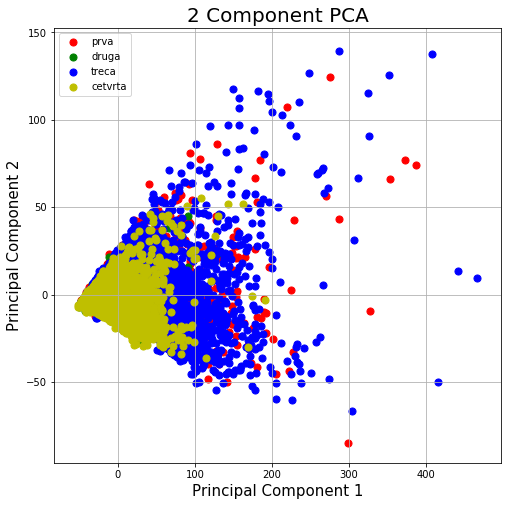
\includegraphics[scale=0.4]{plot_data.png}
\end{center}
\caption{Podaci predstavljeni po klasama u različitim bojama}
\label{fig:podaci}
\end{figure}

\section{Kreiranje modela klasifikacije}
\label{sec:obrada}

Dakle, kao što smo videli u prethodnim poglavljima, podaci su raspoređeni u četiri klase. Prve dve imaju manje, a druge dve znatno više instanci. 

Kod \ref{klase} izlistava vrednosti koje ima atribut klase {\em 'class'}, odnosno ciljni atribut. Kao i što smo očekivali, on može imati četiri vrednosti, zavisno od toga kojoj klasi, odnosno kojoj datoteci na početku, instanca priprada.
\\s
\begin{lstlisting}[caption={Moguće vrednosti atributa 'class'},frame=single, label=klase]
print(df['class'].unique()) #Vrednosti ciljnog atributa: ['prva' 'druga' 'treca' 'cetvrta']
\end{lstlisting}

Na narednom histogramu \ref{fig:klase_hist} možemo videti da je instanci koje pripadaju prvim dvema klasama manje nego instanci koje se nalaze u trećoj i četvrtoj klasi. U prve dve klase imamo po 1567 instanci, a u druge dve po 6483.
\newpage
\begin{figure}[h!]
\begin{center}
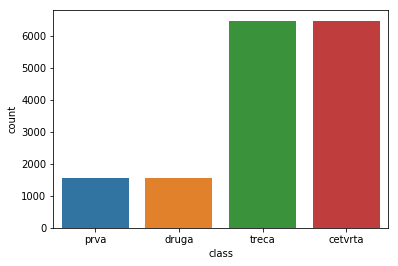
\includegraphics[scale=0.6]{klase_hist.png}
\end{center}
\caption{Količina instanci u prvoj, drugoj, trećoj i četvrtoj klasi}
\label{fig:klase_hist}
\end{figure}

Ova činjenica može ugroziti kreiranje naših modela klasifikacije u nastavku. Javio nam se problem nebalansiranog skupa podataka. Kako bi modeli klasifikacije bili kvalitetni, potrebno je da u svakoj klasi postoji jednak broj instanci. Ukoliko bi podaci ostali nebalansirani moglo bi doći do kreiranja modela koji imaju "lažnu" preciznost. Odnosno, na celokupnom skupu imaju veliki procenat preciznosti, ali kada bi se pogledala matrica konfuzije videli bismo da u klasama koje su "manje popularne", odnosno sadrže manje instanci, dolazi do većeg broja grešaka pri raspoređivanju instanci. Način na koji se ovaj problem može rešiti jesu algoritmi balansiranja skupa podataka (eng.~{\em Re-sampling dataset}). Postoje dva načina balansiranja. Prvi način jeste da se dopune podaci u dvema manjim klasama tako da broj instanci bude jednak broju instanci u većim klasama (eng.~{\em Over-sampling}). Drugi način je da se veće klase smanje tako da u svim klasama bude broj instanci koji je jednak broju instanci u manjim klasama (eng.~{\em Under-sampling}).

\subsection{Podela skupa podataka na trening i test. Balansiranje trening skupa}
Kako bismo mogli da istreniramo različite modele klasifikacije prvo moramo podeliti naš skup podataka na skupove za treniranje modela i kasnije njegovo testiranje. Pošto imamo problem nebalansiranog skupa podataka, koji smo već naveli, potrebno je da izvršimo i balansiranje skupa za trening kako bi mogli da kreiramo model koji je kvalitetan i za manjinske i za većinske klase. 

Za balansiranje podataka upotrebićemo algoritam koji će manje klase dopuniti instancama tako da budu jednake dimenzije kao veće klase (eng.~{\em Over-sampling}). Tehnika koju koristimo na engleskom jeziku naziva se {\em Synthetic minority over-sampling tehnique} - SMOTE. Ona funkcioniše tako što dopunjava manje klase instancama koje kreira na osnovu onih koje već postoje u tim klasama u skupu podataka. Dopunjava ih dok ne dobije broj instanci jednak broju instanci u najvećoj klasi. Na taj način izjednačava se broj instanci u svim klasama.

Naredni kod \ref{split} prikazuje na koji način smo podeliti skup podataka na trening i test skup, i na koji način smo izvršili balansiranje skupa podataka za trening. Važno je napomenuti da je kod algoritma SMOTE upotrebljen argument {\em 'all'} kojim biramo da se sve klase izbalansiraju. Takođe, ispisujemo i dimenziju trening i test skupa pre balansiranja, kao i dimenziju trening skupa nakon izvršenog balansiranja.
\\

\begin{lstlisting}[caption={Podela na trening i test skupove i balansiranje skupa za trening},frame=single, label=split]
import pandas as pd
from sklearn.model_selection import train_test_split
from imblearn.over_sampling import SMOTE
import seaborn as sns


#Ucitavnaje podataka
df = pd.read_csv('data.csv')
print(df.shape)

#X-karakterisike; y-ciljni atribut
X = df.loc[:, df.columns != 'class']
y = df.loc[:,['class']]

#Podela na trening i test skupove:
X_train, X_test, y_train, y_test = train_test_split(X, y, random_state=0)

print("Velicina trening skupa: ")
print(X_train.shape, y_train.shape)
#Velicina trening skupa: 
#X = (12075, 10752) y = (12075, 1)

print("Velicina test skupa:")
print(X_test.shape,y_test.shape)
#Velicina test skupa:
#X = (4025, 10752) y = (4025, 1)


#Kolicina instanci svake klase u trening skupu
print(y_train.groupby('class').size())
#class
#cetvrta    4838
#druga      1199
#prva       1177
#treca      4861

#BALANSIRANJE SKUPA ZA TRENING
smote = SMOTE('all')
X_balanced, y_balanced = smote.fit_sample(X_train,y_train)
#Posto se dobijaju nizovi umesto DataFrame objekta moramo da napravimo DataFrame-ove
y_balanced_df = pd.DataFrame(y_balanced,columns=['class'])
print(y_balanced_df.shape) #Nova dimenzija ciljnog atributa: (19444, 1)

X_balanced_df = pd.DataFrame(X_balanced)
print(X_balanced_df.shape) #Nova dimenzija ostalih atributa: (19444, 10752)

#Kolicina instanci u svakoj klasi nakon balansiranja trening skupa:
print(y_balanced_df.groupby('class').size())
#class
#cetvrta    4861
#druga      4861
#prva       4861
#treca      4861

#Kreiranje histograma sa balansiranim podacima
sns.countplot(y_balanced_df['class'],label="Count")
plt.savefig('klase_balansirane_hist.png', bbox_inches='tight')
\end{lstlisting}

Sada ćemo ponovo histogramom \ref{fig:klase_hist_balansirano} prikazati koliko instanci ima u svakoj klasi u skupu za trening nakon što smo ga izbalansirali.


\begin{figure}[h!]
\begin{center}
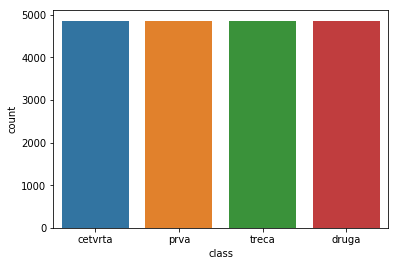
\includegraphics[scale=0.6]{klase_balansirane_hist.png}
\end{center}
\caption{Količina instanci u klasama nakon balansiranja skupa podataka za trening}
\label{fig:klase_hist_balansirano}
\end{figure}

\subsection{Drvo odlučivanja (eng.~{\em Decision tree})}
Prvi algoritam za kreiranje modela klasifikacije koji ćemo prikazati je algoritam drveta odlučivanja (eng.~{\em Decision tree algorithm}). Kako korismo programski jezik Python, tako ćemo koristiti klasu {\em DecisionTreeClassifier} koja nam je u ovom jeziku dostupna. Ova klasa koristi algoritam drveta odlučivanja koji se naziva Stabla za klasifikaciju i regresiju (eng.~{\em Classification and Regression Trees - CART}). 

Prvo ćemo istrenirati model ovim algoritmom pomoću podataka iz nebalansiranog trening skupa, a potom ćemo to uraditi i na blansiranim podacima kako bismo uvideli razliku. 

Naredni kod \ref{tree} prikazuje način na koji smo kreirali modele na pomenuta dva načina. Takođe, i način na koji smo kreirali i vizuelizovali matrice konfuzije. Funkcija koja je korišćena za vizuelizaciju matrice konfuzije {\em plot\_confusion\_matrix} priložena je uz ovaj izveštaj u elektronskom obliku u datoteci {\em 07\_vizuelizacija\_matrice\_konfuzije.py}. U okviru koda pod komentarom može se videti kako izgledaju matrice konfuzije za oba modela i kolike su ukupne preciznosti. Radi lakšeg poređenja u nastavku će biti dat i njihov vizuelni prikaz.
\\
\begin{lstlisting}[caption={Kreiranje modela metodom drveta odlučivanja},frame=single, label=tree]
from sklearn.tree import DecisionTreeClassifier

#Kreiranje modela algoritmom DecisionTreeClassifier na nebalansiranom skupu
clf = DecisionTreeClassifier().fit(X_train, y_train)
y_test_predicted = clf.predict(X_test)

#Cuvanje modela
pickle.dump(clf, open('drvo_sa_nebalansiranim podacima.sav', 'wb'))

#Ispis matrice konfuzije
cm = confusion_matrix(y_test, y_test_predicted)
print(cm)
	#Matrica konfuzije modela kreiranog na nebalansiranom skupu podatka:
	#[[1480   49   28   88]
	# [  47  279   20   22]
	# [  31   26  253   80]
	# [ 150   19   82 1371]]

#Iscrtavanje matrice konfuzije u normalizovanom i nenormalizovanom obliku
plot_confusion_matrix(cm, normalize    = False,
                      target_names = ['cetvrta' , 'druga', 'prva', 'treca'],
                      title = "Confusion Matrix without normalization - 
                      Decission tree (unbalanced dataset)")

plot_confusion_matrix(cm, normalize    = True,
                      target_names = ['cetvrta' , 'druga', 'prva', 'treca'],
                      title = "Confusion Matrix with normalization - 
                      Decision tree (unbalanced dataset)")

#Ispis preciznosti modela kreiranom na nebalansiranom skupi
print("Preciznost na nebalansiranom skupu: " , clf.score(X_test, y_test))
	#Preciznost na nebalansiranom skupu:  0.8404968944099379



#Kreiranje modela algoritmom Drveta odlucivanja na balansiranom skupu podataka
clf_balanced = DecisionTreeClassifier().fit(X_balanced_df, y_balanced_df)
y_test_predicted_balanced = clf_balanced.predict(X_test)

#Cuvanje modela
pickle.dump(clf_balanced, open('drvo_sa_balansiranim podacima.sav', 'wb'))

#Ispis matrice konfuzije
cm_balanced = confusion_matrix(y_test, y_test_predicted_balanced)
print(cm_balanced)
	#Matrica konfuzije modela kreiranom na balansiranom skupu podatka:
	#[[1449   56   37  103]
	# [  38  306   20    4]
	# [  31   29  293   37]
	# [ 124   12   92 1394]]

#Iscrtavanje matrice konfuzije u normlizovanom i nenormalizovanom obliku
plot_confusion_matrix(cm_balanced, normalize    = False,
                      target_names = ['cetvrta' , 'druga', 'prva', 'treca'],
                      title = "Confusion Matrix without normalization - 
                      Decision tree (balanced dataset)")

plot_confusion_matrix(cm_balanced, normalize    = True,
                      target_names = ['cetvrta' , 'druga', 'prva', 'treca'],
                      title = "Confusion Matrix with normalization - 
                      Decision tree (balanced dataset)")

#Ispis preciznosti modela kreiranom na balansiranom skupu
print("Preciznost na balansiranom skupu:",clf_balanced.score(X_test, y_test))
	#Preciznost na balansiranom skupu: 0.8551552795031055
\end{lstlisting}

Kada smo kreirali oba modela možemo prikazati matrice konfuzije koje smo dobili. Za ove modele biće prikazane matrice konfuzije u dva oblika - normalizovanom i nenormalizovanom. 

Na slikama \ref{fig:mat_nebalansirana1} i \ref{fig:mat_nebalansirana2} prikazane su matrice konfuzije za model dobijen CART algoritmom nad nebalansiranim trening podacima. Takođe, na dnu se može videti i preciznost modela, kao i procenat promašaja.

\begin{figure}[h!]
\begin{center}
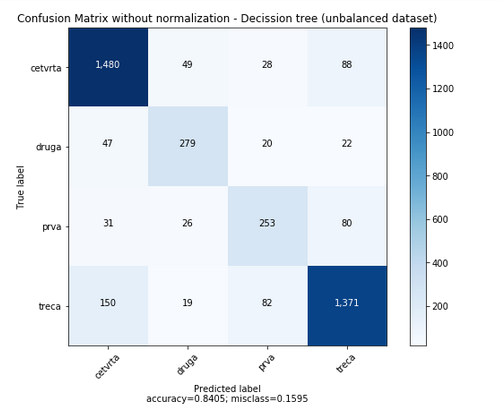
\includegraphics[scale=0.55]{drvo-nebalansirani-nenormalizovana-mat-konf.png}
\end{center}
\caption{Nenormalizovana matrica konfuzije modela dobijenog drvetom odlučivanja nad nebalansiranim trening podacima. Preciznost i broj promošaja}
\label{fig:mat_nebalansirana1}
\end{figure}

\newpage

\begin{figure}[h!]
\begin{center}
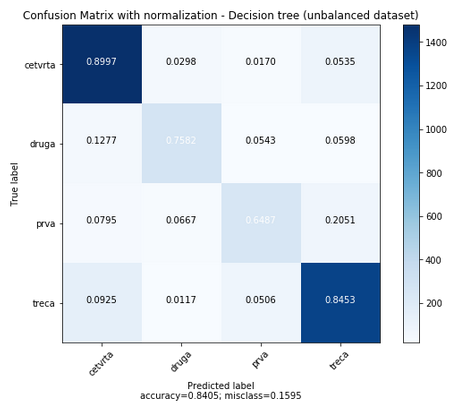
\includegraphics[scale=0.55]{drvo-nebalansirani-normalizovana-mat-konf.png}
\end{center}
\caption{Normalizovana matrica konfuzije modela dobijenog drvetom odlučivanja nad nebalansiranim trening podacima. Preciznost i broj promašaja}
\label{fig:mat_nebalansirana2}
\end{figure}

Na slikama \ref{fig:mat_balansirana1} i \ref{fig:mat_balansirana2} prikazane su matrice konfuzije za model dobijen CART algoritmom nad balansiranim trening podacima. Takođe, na dnu se može videti i preciznost modela, kao i procenat promašaja.

\begin{figure}[h!]
\begin{center}
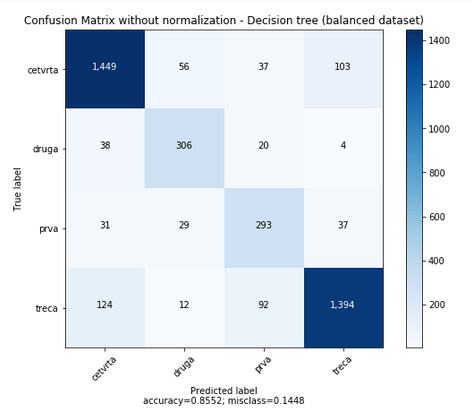
\includegraphics[scale=0.5]{drvo-balansirano-nenormalizovana-mat-konf.png}
\end{center}
\caption{Nenormalizovana matrica konfuzije modela dobijenog drvetom odlučivanja nad balansiranim trening podacima. Preciznost i broj promašaja}
\label{fig:mat_balansirana1}
\end{figure}


\begin{figure}[h!]
\begin{center}
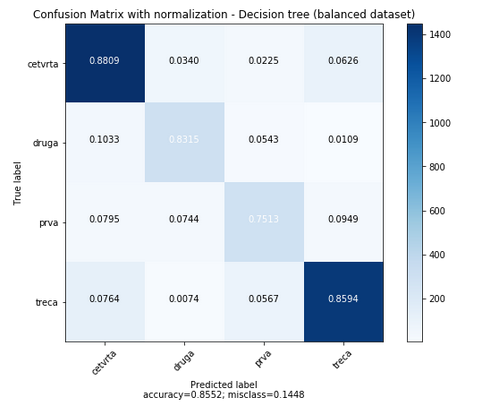
\includegraphics[scale=0.5]{drvo-balansirano-normalizovana-mat-konf.png}
\end{center}
\caption{Normalizovana matrica konfuzije modela dobijenog drvetom odlučivanja nad balansiranim trening podacima. Preciznost i broj promašaja}
\label{fig:mat_balansirana2}
\end{figure}

Kada imamo vizuelni prikaz kvaliteta oba modela možemo primetiti da je u manjim klasama dosta veća preciznost kada je za treniranje korišćen balansirani skup podataka za trening nego kada klase nisu bile balansirane. Takođe se može primetiti da je celokupna preciznost u oba slučaja slična, ali se ipak povećala kada je korišćen balansiran skup podataka. Ovo je situacija sa "lažnom preciznošću" koju smo ranije pomenuli.

Što se tiče samog modela, ispostavlja se da je ovaj model za naš skup podataka prilično dobar. Preciznost iznosi 0.855. Treniranje je trajalo nekoliko minuta što je veoma dobro. Ali ćemo istrenirati još neke modele nad našim podacima kako bismo ispitali da li može i bolje od ovoga. 
\\

U narednim modelima koje ćemo kreirati koristićemo samo balansiran skup trening podataka, jer smo se uverili na ovom primeru da on daje bolje rezultate. Takođe, možemo odabrati bilo koji od ova dva prikaza matrice konfuzije, jer oba daju jasnu sliku koliko je kreirani model dobar. Mi ćemo se odlučiti za normalizovanu matricu konfuzije u vizuelnom prikazu jer nam on odmah procentualno daje uvid koliko je instanci u svakoj klasi dobro raspoređeno.

\subsection{Logistička regresija (eng.~{\em Logistic regression})}
Klasifikator koji treniramo nakon modela dobijenog prethodnim algoritmom, je model dobijen Logistickom regresijom (eng.~{\em Logistic regression}). Ovaj model takođe postoji kao ugrađena biblioteka u programskom jeziku Python i trenira se pomoću klase {\em LogisticRegression}. Za treniranje koristimo balansirani trening skup podataka.

Naredni kod \ref{logreg} prikazuje način na koji smo istrenirali model, kao i rezultate koje je on dao prikazane u okviru koda pod komentarom. Matricu konfuzije vizuelno prikazujemo u normalizovanom obliku.
\\
\begin{lstlisting}[caption={Kreiranje modela logističkom regresijom i prikaz rezultata},frame=single, label=logreg]
from sklearn.linear_model import LogisticRegression

#Kreiranje modela logistickom regresijom
logreg = LogisticRegression()
logreg.fit(X_balanced, y_balanced)

#Cuvanje modela
pickle.dump(logreg, open('logreg_model.sav', 'wb'))

#Ispis matrice konfuzije:
y_predicted = logreg.predict(X_test)
cm_logreg = confusion_matrix(y_test, y_predicted)
print(cm_logreg)

	#Matrica konfuzije:
	#[[1641    4    0    0]
	#[  12  355    1    0]
	#[   0    2  372   16]
	#[  10    0    8 1604]]

#Vizuelni prikaz matrice konfuzije:
plot_confusion_matrix(cm_logreg, normalize    = True,
                      target_names = ['cetvrta' , 'druga', 'prva', 'treca'],
                      title = "Confusion Matrix -Logistic Regression")

#Preciznost modela:
print("Preciznost modela dobijenog logistickom regresijom:",logreg.score(X_test, y_test))
	#Preciznost modela dobijenog logistickom regresijom: 0.986832298136646
\end{lstlisting}

Na slici \ref{fig:logreg_mk} vizuelizovana je matrica konfuzije modela dobijenog logističkom regresijom. Možemo primetiti da je ovaj model znatno bolji od modela dobijenog drvetom odlučivanja na balansiranom trening skupu. Ukupna preciznost je veća i iznosi 0,99 , a i preciznost po klasama zasebno je znatno bolja. Treniranje ovog modela trajalo je oko 15 minuta što je dobro za naš skup podataka.
%\newpage

\begin{figure}[h!]
\begin{center}
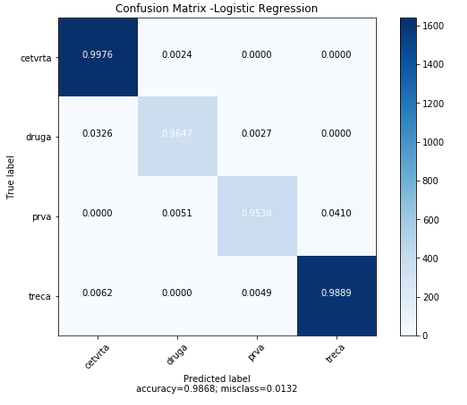
\includegraphics[scale=0.55]{logisticka_regresija_matrica_konfuzije.png}
\end{center}
\caption{Matrica konfuzije modela dobijenog logističkom regresijom. Preciznost i broj promašaja}
\label{fig:logreg_mk}
\end{figure}



\subsection{K najbližih suseda (eng.~{\em K-Nearest Neighbors})}
Sledeći metod koji koristimo za treniranje modela klasifikacije nad našim podacima je metod k najbližih suseda (eng.~{\em K-Nearest Neighbors}). Kreirali smo više modela za različite vrednosti parametra k, koji predstavlja broj najbližih suseda koje će algoritam tražiti. Koristili smo sledeće vrednosti: 2,4,5,8,10 i 25. Tokom treniranja primećeno je da kada se parametar {\em algorithm} postavi na vrednost {\em 'brute'} treniranje traje znatno kraće, kao i računanje matrice konfuzije i preciznosti. Zbog toga je u svim slučajevima korišćen ovaj algoritam umesto automatskog. Rezultati su i sa automatskim identični. 

Skoro svi modeli dali su približno slične rezultate. Krenuli smo od nižih vrednosti za k. Obzirom da smo za k = 2 i k = 4 dobili slične matrice konfuzije, povećali smo korak uvećanja za k. Pošto se ništa znatno nije promenilo, tj. preciznsot se i dalje kretala oko 0,69 , pokušali smo da uvećamo dosta više parametar. Međutim, za k = 25 dobijamo još nižu preciznost koja iznosi 0,68. Na kraju, pošto je model za k = 4 dao do sada najvišu preciznost od 0,7 kreirali smo još model i za k = 5 i ovaj model daje definitivno nabolji rezultat. Njegova preciznost je 0,72. Zbog toga ćemo taj model predstaviti u izveštaju i prikazati njegovu matricu konfuzije, dok ćemo rezultate ostalih modela priložiti u elektonrkom formatu.

Naredni kod \ref{knn} prikazuje način na koji smo kreirali model ovom metodom za k = 5. U jeziku Python postoji biblioteka za ovaj model koja sadrži klasu {\em KNeighborsClassifier} pomoću koje ćemo napraviti klasifikator. Pramaetrom {\em n\_neighbors=5} podesili smo koju vrednost za k želimo. Čak nismo ni morali da navodimo jer je podrazumevana vrednost ovog parametra baš 5. Takođe, naredni kod ispisuje matricu konfuzije modela, preciznost i poziva funkciju za vizuelizaciju matrice konfuzije.
\\
\begin{lstlisting}[caption={Kreiranje modela algoritmom kNN i prikaz rezultata},frame=single, label=knn]
from sklearn.neighbors import KNeighborsClassifier

#Kreiranje modela metodom k najbliyih suseda (k = 5)
knn = KNeighborsClassifier(n_neighbors=5,metric='minkowski',algorithm = 'brute')
knn.fit(X_balanced, y_balanced)

#Cuvanje modela
pickle.dump(knn, open('knn_k_5_minkowski_brute.sav', 'wb'))

#Kreiranje matrice konfuzije
y_predicted_knn = knn.predict(X_test)
cm_knn = confusion_matrix(y_test, y_predicted_knn)
print(cm_knn)
    #Matrica konfuzije
    #[[1251  326   25   43]
 	#[  31  324   13    0]
 	#[   8   50  319   13]
 	#[ 330   59  249  984]]

print("Preciznost modela dobijenog metodom k najblizih suseda:",knn.score(X_test, y_test))
    #"Preciznost modela dobijenog metodom k najblizih suseda:   0.7150310559006211

#Vizuelizacija matrice konfuzije
plot_confusion_matrix(cm_knn, normalize    = True,
                      target_names = ['cetvrta' , 'druga', 'prva', 'treca'],
                      title  = "Confusion Matrix - 
                      kNN (k = 5; metric = 'minkowski', algorithm = 'brute')")
\end{lstlisting}

Na slici \ref{fig:kNN} prikazana je normalizovana matrica konfuzije dobijena kNN metodom za k = 5. Od svih dosadašnjih algoritama ovaj se na našem skupu najlošije pokazao. Preciznost je najniža do sada i iznosi 0,72. Takođe, i preciznost po klasama je znatno lošija od ranijih. U trećoj klasi se javljalo najviše loše raspoređenih instanci za sve parametre k koje smo koristili. Treniranje modela trajalo je relativno kratko.
\newpage

\begin{figure}[h!]
\begin{center}
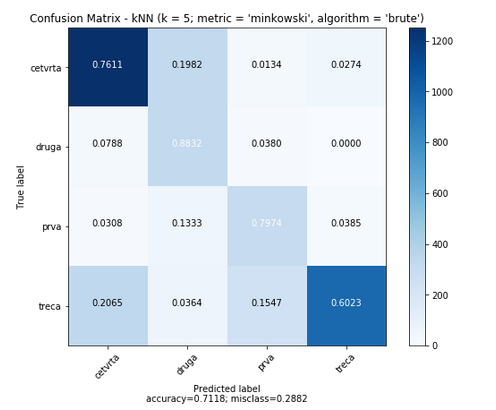
\includegraphics[scale=0.55]{kNN_k_5.png}
\end{center}
\caption{Matrica konfuzije modela dobijenog metodom k najbližih suseda}
\label{fig:kNN}
\end{figure}


\subsection{Naivni Bajesov metod (eng.~{\em Naive Bayes})}
Model koji ćemo sada pokušati da primenimo na naš skup podataka kako bismo dobili klasifikator je model koji je zasnovan na Bajesovom pravilu.
Bajesovo pravilo:
\[
    P(h|D) = \frac{P(D|h)*P(h)}{P(D)}
\]
Ovaj model koristi dve "naivne" predpostavke nad atributima modela. Odatle i njegov naziv Naivni Bajesov metod (eng.~{\em Naive Bayes}). Prva pretpostavka je da su svi atributi podjednako važni za model što u našem skupu podataka i jeste slučaj. Druga pretpostavka je da atributi nisu statički međusobno zavisni. Ovo, takođe, ispunjava naš skup podataka obzirom da nam ni jedna vrednost atributa ne govori ništa o nekoj drugoj vrednosti. Svaki atribut predstavlja gen za sebe. Za ovaj model važi i da on ima visoku preciznost i brzinu na velikim skupovima podataka. Zbog svih ovih pretpostavki, koje se podudaraju sa našim podacima, primenićemo ga na naš skup.

Jezik Python, u kome radimo istraživanje, i za ovaj algoritam ima ugrađenu biblioteku. Tako da model treniramo pomoću klase {\em GaussianNB}. Naredni kod \ref{nbm} prikazuje način na koji smo istrenirali ovaj model. Prvo smo istrenirali model koristeći balansirani trening skup podataka. Međutim, dobija se dosta niža preciznost, i ukupna i pojedinačno u svakoj klasi. Zbog toga, ipak, treniramo model i na nebalansiranom trening skupu kako bismo uporedili rezultat. Iznenađujuće, ovaj model daje mnogo bolji rezultat nego prethodni. 
\\

\begin{lstlisting}[caption={Kreiranje modela Naivnim Bajesovim algoritmom nad balansiranim i nebalansiranim trening podacima},frame=single, label=nbm]
from sklearn.naive_bayes import GaussianNB

#Naivni Bajesov algoritam nad balansiranim trening skupom
gnb = GaussianNB()
gnb.fit(X_balanced_df, y_balanced_df)

#Cuvanje modela
pickle.dump(gnb, open('naivni_bajes_balansirani_podaci.sav', 'wb'))

#Kreiranje i ispis matrice konfuzije
y_predicted_gnb = gnb.predict(X_test)
cm_gnb = confusion_matrix(y_test, y_predicted_gnb)
print(cm_gnb)
	#Matrice konfuzija modela dobijenog nad nebalansiranim trening skupom
	#[[1022  536   57   30]
	#[  21  299   42    6]
	#[   0    0  389    1]
	#[   2    1  351 1268]]

print("Preciznost modela nad balansiranim podacima:",gnb.score(X_test, y_test))
	#Preciznost modela nad balansiranim podacima: 0.7398757763975156

#Vizuelizacija matrice konfuzije:
plot_confusion_matrix(cm_gnb, normalize = True,
                      target_names = ['cetvrta' , 'druga', 'prva', 'treca'],
                      title = "Confusion Matrix - Naive Bayes (balanced dataset)")


    
#Naivni Bajesov algoritam nad nebalansiranim trening skupom
gnb = GaussianNB()
gnb.fit(X_train, y_train)

#Cuvanje modela
pickle.dump(gnb, open('naivni_bajes_nebalansirani_podaci.sav', 'wb'))

#Kreiranje i ispis matrice konfuzije
y_predicted_gnb = gnb.predict(X_test)
cm_gnb = confusion_matrix(y_test, y_predicted_gnb)
print(cm_gnb)
	#Matrice konfuzija modela dobijenog nad nebalansiranim trening skupom:
	#[[1553   11    1   80]
	# [   0  346    1   21]
	# [   0    0  373   17]
	# [   3    2    3 1614]]

print("Preciznost modela nad nebalansiranim podacima:",gnb.score(X_test, y_test))
	#Preciznost modela nad nebalansiranim podacima: 0.9654658385093168

#Vizuelizacija matrice konfuzije:
plot_confusion_matrix(cm_gnb, normalize = True,
                      target_names = ['cetvrta' , 'druga', 'prva', 'treca'],
                      title = "Confusion Matrix - Naive Bayes (unbalanced dataset)")

\end{lstlisting}

Na slikama \ref{fig:bajes1} i \ref{fig:bajes2} prikazujemo normalizovane matrice konfuzije za oba kreirana modela. Možemo videti preciznosti i pojedinačno na svakoj klasi. I u manjinskim, i u većinskim klasama preciznost je mnogo veća kod modela kreiranog na nebalansiranom trening skupu. Pretpostavka zbog koje se ovo moglo dogoditi je zbog toga kako funkcioniše SMOTE algoritam za balansiranje skupa podataka. Ovaj algoritam je dodao instance na osnovu već postojećih i moguće je da su se stvroile određene zavisnosti među atributima. Naivni Bajesov algoritam pretpostavlja nezavisnost, ali može raditi i nad međusobno zavisnim atributima. 

\begin{figure}[h!]
\begin{center}
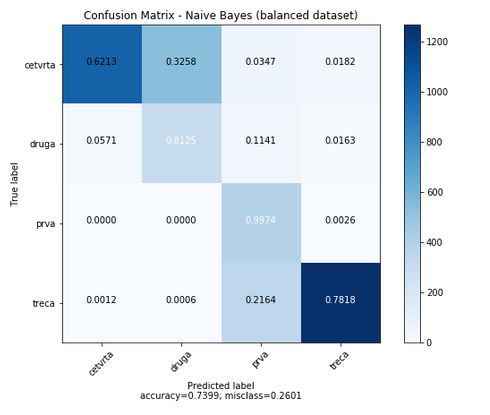
\includegraphics[scale=0.5]{bajes_balansirani_skup.png}
\end{center}
\caption{Matrica konfuzije modela dobijenog Naivnim Bajesovim algoritmom nad balansiranim trening podacima}
\label{fig:bajes1}
\end{figure}

\newpage

\begin{figure}[h!]
\begin{center}
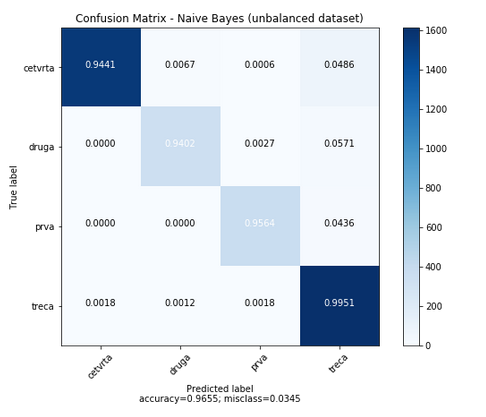
\includegraphics[scale=0.5]{bajes_nebalansirani_skup.png}
\end{center}
\caption{Matrica konfuzije modela dobijenog Naivnim Bajesovim algoritmom nad nebalansiranim trening podacima}
\label{fig:bajes2}
\end{figure}

Dakle, model koji je ovim metodom dao bolje rezultate je izrazito dobar za naš skup podataka. Treniranje modela trajalo je kratko i vrlo brzo smo dobili rezultate. Ukupna preciznost je 0,97, a i preciznosti u pojedinačnim klasama su visoke.

\subsection{Metod potpornih vektora (eng.~{\em Support Vector Machine})}
Poslednji metod kojim ćemo napraviti klasifikator na osnovu balansiranog trening skupa je metod potpornih vektora (eng.~{\em Support Vector Machine - SVM}). Kako bismo dobili što bolji model koristili smo linearni, polinomijalni i RBF ({\em Radial Basis Function}) kernel. Najbolje rezultate dao nam je model koji je treniran pomoću linearnog kernela. Zbog toga ćemo izdvojiti kod kojim je ovaj model kreiran i prikazati njegove rezultate. Model dobijen ovim algoritmom sa polinomijalnim kernelom biće dodat uz izveštaj u eletronskom formatu, kao i njegovi rezultati. Što se tiče modela sa RBF kernelom, njegovo treniranje trajalo je više od sat vremena. Kako smo za obradu koristili besplatno okruženje za rad putem web pretraživača, zbog trajanja sesije model nismo uspeli da istreniramo do kraja.

Kod \ref{svm} prikazuje način kreiranja modela SVM algoritmom koji koristi linearni kernel. Programski jezik Python i za ovaj algoritam ima biblioteku i u okviru nje klasu {\em SVC} pomoću koje treniramo model. U okviru metoda koristimo parametar {\em kernel = 'linear'} kako bismo definisali kernel koji želimo. U kodu pod komentarom će biti ispisana i matrica konfuzije kao i preciznost modela. Takođe, biće pozvana funkcija za vizuelizaciju matrice konfuzije.
\\
\begin{lstlisting}[caption={Kreiranje modela algoritmom SVM sa linearnim kernelom i prikaz rezultata},frame=single, label=svm]
from sklearn.svm import SVC

#Kreiranje modela klasifikacije
svm = SVC(kernel = 'linear')
svm.fit(X_balanced_df, y_balanced_df)

#Cuvanje modela
pickle.dump(svm, open('SVM_linear.sav', 'wb')

#Kreiranje matrice konfuzije
y_predicted_svm = svm.predict(X_test)
cm_svm = confusion_matrix(y_test, y_predicted_svm)
print(cm_svm)
	#Matrica konfuzije:
	#[[1637    8    0    0]
	#[  16  351    1    0]
	#[   4    0  369   17]
	#[  11    0    7 1604]]

print("Preciznost modela dobijenog SVM algoritmom sa linearnim kernelom: ",svm.score(X_test, y_test))
	#Preciznost modela dobijenog SVM algoritmom sa linearnim kernelom: 0.9840993788819876

#Vizuelni prikaz normalizovane matrice konfuzije
plot_confusion_matrix(cm_svm, normalize = True,
                      target_names = ['cetvrta' , 'druga', 'prva', 'treca'],
                      title = "Confusion Matrix - SVM (kernel = 'linear')")
\end{lstlisting}

Na slici \ref{fig:svm} se vidi normalizovana matrica konfuzije dobijena na prethodno opisan način. U dnu slike vidi se i preciznost modela koja iznosi 0,98. Takođe je prikazan broj promašaja klasifikatora. Ovaj model je veoma dobar za naš skup podataka. Treniranje je trajalo nešto duže, oko 15 minuta.

\begin{figure}[h!]
\begin{center}
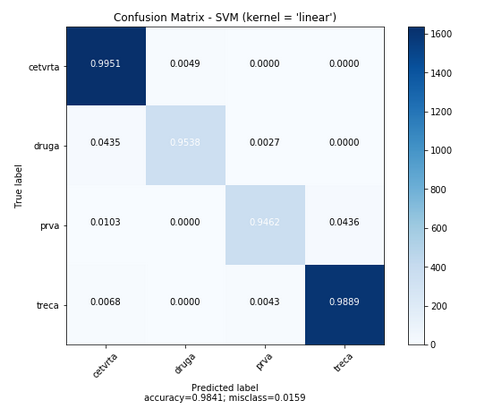
\includegraphics[scale=0.55]{svm_linear.png}
\end{center}
\caption{Matrica konfuzije modela dobijenog SVM algoritmom sa linearnim kernelom}
\label{fig:svm}
\end{figure}


\section{Zaključak}
\label{sec:zakljucak}
Ovim radom prikazano je nekoliko najkorišćenijih modela klasifikacije danas. Najkvalitetniji model za naš skup podataka bio je model kreiran metodom logističke regresije. Preciznost ovog modela je čak 0,99. Samo treniranje modela izvršeno je veoma brzo. 

Pored ovih algoritama postoji još puno metoda koje su se mogle primeniti na ovaj skup podataka. To bi bila ideja za dalje istraživanje podataka o Limfoblastoidnim ćelijama.

Uz ovaj izveštaj, kao rezultati istraživanja, priloženi su i celokupni kodovi koji su implementirani u {\em .py} formatu. Zatim, sve slike kreiranih vizuelnih prikaza u {\em .png} formatu. Takođe , i rezultati, u {\em .txt} formatu, svakog kreiranog modela klasifikacije koji sadrže matricu konfuzije i preciznost modela. U materijalima priloženi su i sami kreirani modeli u {\em .sav} formatu.

\newpage

\addcontentsline{toc}{section}{Literatura}
\appendix
\bibliography{seminarski} 
\bibliographystyle{plain}



\end{document}
